%%%%% Magnetisches Feld %%%%%
%%  %%


%Some sample text to be displayed above the first subsection

%\subsection{Prinzip}

%Ein Zyklotron besteht aus Zwei hohlen, halbzylindrischen und Duanden an denen eine Spannung mit unterschiedlichem Vorzeichen anliegt, und darüber bzw. darunter liegende Magneten, die ein homogenes Magnetfeld erzeugen. Zudem gibt es einen Einlass und einen Auslass für Teilchen.

%\begin{wrapfigure}{r}{0.4\textwidth} \label{Zyklo}
%
%	\vspace{-10pt}
%	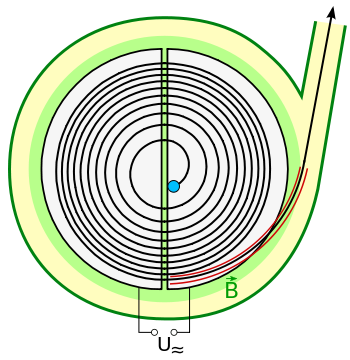
\includegraphics[width=0.35\textwidth]{Zyklotron_Prinzipskizze02.png}
%	\vspace{-13pt}
%	\caption{Prinzipskizze eines Zyklotrons}
%	\vspace{-5pt}	
%	
%\end{wrapfigure}

%\subsubsection{Anwendung}

% Some Formula:

%\begin{equation}
%	x= \frac{y \cdot 13 \pi z}
%			{\cos \alpha}
%\end{equation}

%%%%%%%%%%%%%%%%%%%%%%%
% Eigentlicher Beginn %
%%%%%%%%%%%%%%%%%%%%%%%

\subsection{Geladenes Teilchen}

Die Lorentzkraft wirkt auf jedes geladene, in einem Magnetfeld bewegte Teilchen, wenn sich dieses Teilchen nicht parallel zu den Feldlinien bewegt. Die Lorentzkraft ist abhängig von der Flussdichte des Magnetfeldes, der Ladung und Geschwindigkeit des Teilchens und von dem Winkel zu den Feldlinien. Im Folgenden werden jedoch nur noch Fälle betrachtet, bei denen sich Teilchen senkrecht zu den Feldlinien bewegen.


\subsection{Stromdurchflossener Leiter}

Durch einen stromdurchflossenen Leiter fließen Elektronen vom Minuspol zum Pluspol. Da Elektronen negativ geladene Teilchen sind, wirkt auch in diesem Fall die Lorentzkraft auf den Leiter, wenn sich der Leiter in einem magnetischen Feld befindet.

%Cue for schwierige Aufgabe: Wie groß Kraft auf geraden Leiter, auf den Stromstärke etc...

\subsection{Handregeln}

\begin{figure}[h!]
	\centering
	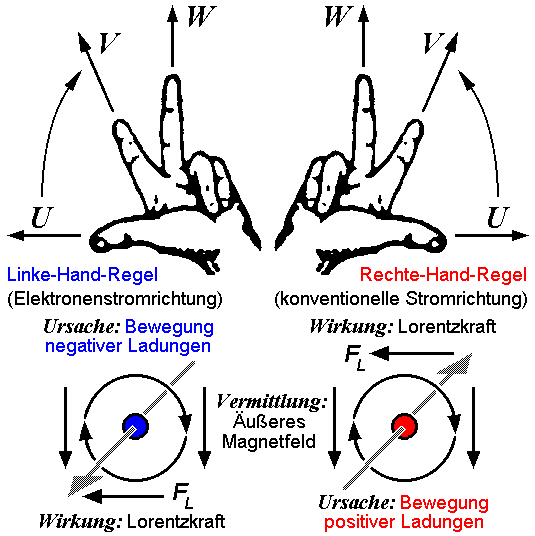
\includegraphics[width=0.65\textwidth]{Handregeln}
	\caption{Die beiden Handregeln für negative und die positive Teilchen. Die Linke gilt zudem für die physikalische und die Rechte für die Technische Stromrichtung. U: Ursache, V: Vermittlung, W: Wirkung}
	\label{fig:Handregeln}
\end{figure}

Bei der Richtung der Lorentzkraft auf ein negativ geladenes Teilchen, das sich senkrecht zu den Feldlinien eines magnetischen Feldes bewegt, gilt die linke Handregel. Bei dieser werden Daumen, Zeige- und Mittelfinger der linken Hand abgespreizt, sodass sie der Zeichnung \ref{fig:Handregeln}\footnote{„UVWREGEL new“ von UVWREGEL.png: Qniemiec 19:15, 14. Jan. 2011 (CET).Original uploader was Qniemiec at de.wikipediaderivative work: Qniemiec (talk) - UVWREGEL.png. Lizenziert unter CC BY-SA 3.0 über Wikimedia Commons - \url{https://commons.wikimedia.org/wiki/File:UVWREGEL_new.png}} entsprechen. Dann bezeichnet der Daumen die Richtung des Teilchens, der Zeigefinger folgt der Richtung des Magnetfeldes und der Mittelfinder zeigt schlussendlich die Richtung der Lorentzkraft an. Für die Kraft auf einen Leiter, der senkrecht in einem Magnetfeld steht, gilt dieselbe Regel wobei der Daumen die die physikalische Stromrichtung anzeigt.

Für ein positives Teilchen oder die technische Stromrichtung in einem Leiter kommt die rechte Hand zum Einsatz; die Regel für die Bezeichnung der Finger bleibt gleich.


\subsection{Gleichung} \label{subsec:BLorentzDefinition}

Der Betrag der Lorentzkraft lässt sich wie folgt berechnen:

\begin{align} \label{eq:Lorentzkraft}
\begin{split}
	F_{Lr} = q \cdot B \cdot v
\end{split}
\end{align}

\noindent Interessant ist, dass die Lorentzkraft nicht nur von der Ladung, sondern auch von der Geschwindigkeit des Teilchens abhängig ist. Dies macht man sich z.B. im Massenspektrometer (Siehe: \referenz{sec:Massenspektrometer}) oder im Wien'schen Filter (Siehe: \referenz{sec:Wien}) zu Nutze.

Aus der Lorentzkraft lässt sich auch die Flussdichte $B$ definieren: Die Flussdichte ordnet jedem bewegten, geladenen Körper eine Kraft (die Lorentzkraft) zu:

\begin{align} \label{eq:Flussdichte}
\begin{split}
	\vec{B} = \frac{\vec{F}_{Lr}}{q \cdot \vec{v}}
\end{split}
\end{align}






